% Neural networks are tight!

% TODO: move future tense to past tense

\section{Motivation}
\label{sec:introduction}
In a 2016 survey by Springer \cite{baker_1500_2016}, 52\% of scientists across multiple fields of study reported that they felt there was a ``significant crisis'' in the reproducibility of published research. Another 38\% felt there was a ``slight crisis.'' This ``reproducibility crisis'' describes the consensus among the scientific community that an outsized portion of published research is not reproduced. ``Our analysis...suggests
a large proportion of CS research faces
the same threats to replication as those
encountered in other areas,'' writes Cockburn, et al in a recent edition of \textit{Communications of the ACM}. Non-reproducible research is problematic because (1) it is more challenging for other researchers to use the research technology in their own projects, and (2) there exists no independent verification of the research's validity. Therefore, reproducing research should be important to the scientific community. 

\begin{figure}
    \centering
    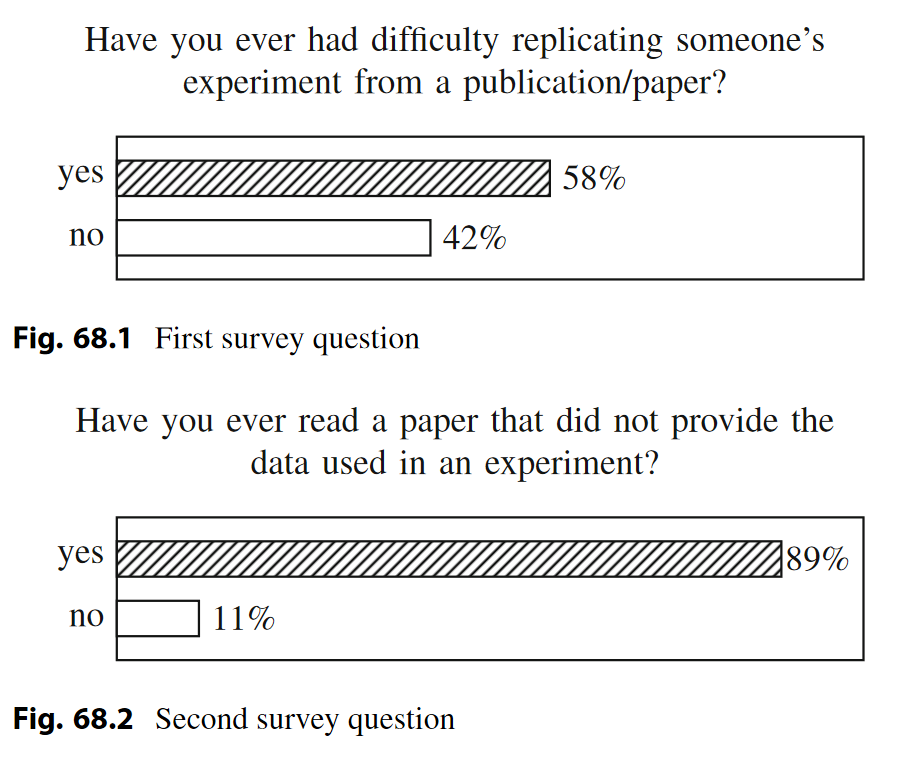
\includegraphics[width=\linewidth]{images/IT.PNG}
    \caption{ (image credit ITNG 2020 \cite{cacho_state_2020})}
    \label{fig:nature_magazine_reproducibility_figure}
    \vspace{-0.2in}
\end{figure}

Unfortunately, few replication studies (formal studies that attempt to independently reproduce an existing work and document its results) are attempted. This is due to many reasons, including: reproducing a study might be expensive, attempting to question an author might be seen as malicious or reflecting incompetence, spending the time to reproduce a study may not further one's own research, etc. Additionally, scientists unable to reproduce work might be inclined to write off a failure as some personal mistake and move on. Incentives to publish positive replications are already low; journals can be even more reluctant to publish negative findings \cite{cacho_state_2020}. This all contributes to the ``file drawer effect'': replication work that would otherwise be useful goes unpublished \cite{cockburn_threats_2020}.  Therefore, the lack of replication studies continues.
% ``When work does not reproduce, researchers often assume there is a perfectly valid (and probably boring) reason. What's more, ,'' writes \textit{Nature} editor Monya Baker \cite{baker_1500_2016}. T

 By performing the replication study ourselves, we wished to contribute to the software engineering community and add a positive effect to mitigate the ``reproducibility crisis.'' Hopefully, our replication study motivates other software engineers to participate in replication studies. Narrowly, we attempt to give a better insight to other researchers who seek to implement DeepBugs into their system. 
